% Options for packages loaded elsewhere
\PassOptionsToPackage{unicode}{hyperref}
\PassOptionsToPackage{hyphens}{url}
%
\documentclass[
]{article}
\usepackage{lmodern}
\usepackage{amssymb,amsmath}
\usepackage{ifxetex,ifluatex}
\ifnum 0\ifxetex 1\fi\ifluatex 1\fi=0 % if pdftex
  \usepackage[T1]{fontenc}
  \usepackage[utf8]{inputenc}
  \usepackage{textcomp} % provide euro and other symbols
\else % if luatex or xetex
  \usepackage{unicode-math}
  \defaultfontfeatures{Scale=MatchLowercase}
  \defaultfontfeatures[\rmfamily]{Ligatures=TeX,Scale=1}
\fi
% Use upquote if available, for straight quotes in verbatim environments
\IfFileExists{upquote.sty}{\usepackage{upquote}}{}
\IfFileExists{microtype.sty}{% use microtype if available
  \usepackage[]{microtype}
  \UseMicrotypeSet[protrusion]{basicmath} % disable protrusion for tt fonts
}{}
\makeatletter
\@ifundefined{KOMAClassName}{% if non-KOMA class
  \IfFileExists{parskip.sty}{%
    \usepackage{parskip}
  }{% else
    \setlength{\parindent}{0pt}
    \setlength{\parskip}{6pt plus 2pt minus 1pt}}
}{% if KOMA class
  \KOMAoptions{parskip=half}}
\makeatother
\usepackage{xcolor}
\IfFileExists{xurl.sty}{\usepackage{xurl}}{} % add URL line breaks if available
\IfFileExists{bookmark.sty}{\usepackage{bookmark}}{\usepackage{hyperref}}
\hypersetup{
  pdftitle={Tweet Thread},
  hidelinks,
  pdfcreator={LaTeX via pandoc}}
\urlstyle{same} % disable monospaced font for URLs
\usepackage[margin=1in]{geometry}
\usepackage{graphicx}
\makeatletter
\def\maxwidth{\ifdim\Gin@nat@width>\linewidth\linewidth\else\Gin@nat@width\fi}
\def\maxheight{\ifdim\Gin@nat@height>\textheight\textheight\else\Gin@nat@height\fi}
\makeatother
% Scale images if necessary, so that they will not overflow the page
% margins by default, and it is still possible to overwrite the defaults
% using explicit options in \includegraphics[width, height, ...]{}
\setkeys{Gin}{width=\maxwidth,height=\maxheight,keepaspectratio}
% Set default figure placement to htbp
\makeatletter
\def\fps@figure{htbp}
\makeatother
\setlength{\emergencystretch}{3em} % prevent overfull lines
\providecommand{\tightlist}{%
  \setlength{\itemsep}{0pt}\setlength{\parskip}{0pt}}
\setcounter{secnumdepth}{-\maxdimen} % remove section numbering
\ifluatex
  \usepackage{selnolig}  % disable illegal ligatures
\fi

\title{Tweet Thread}
\author{}
\date{\vspace{-2.5em}}

\begin{document}
\maketitle

\hypertarget{tweet-1}{%
\section{Tweet 1}\label{tweet-1}}

Hi Argo community! I want to introduce you to a newly developed R
package, argoFloats. This package was created by myself, Dan Kelley, and
Jaimie Harbin to provide tools for downloading and analyzing collections
of oceanographic Argo float datasets.
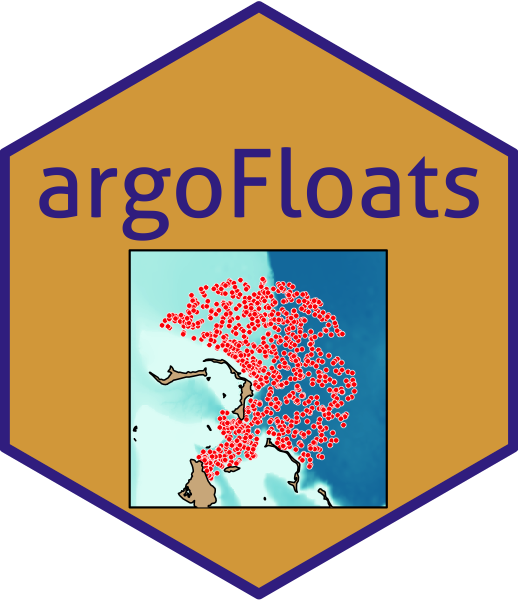
\includegraphics{../18_tweets/argoFloats_logo_06.png}

\hypertarget{tweet-2}{%
\section{Tweet 2}\label{tweet-2}}

argoFloats has an easy-to-follow work flow, to allow the users to
effectively access, download, and read Argo data. It targets both
experienced and new R users.

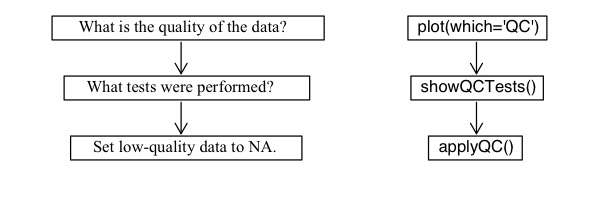
\includegraphics{../../../vignettes/flowchart.png}

\hypertarget{tweet-3}{%
\section{Tweet 3}\label{tweet-3}}

To get familiar with argoFloats, check out the user website,
\url{https://argocanada.github.io/argoFloats/index.html}, or developer
website \url{https://github.com/ArgoCanada/argoFloats} for more advanced
R users.

\hypertarget{tweet-4}{%
\section{Tweet 4}\label{tweet-4}}

Users can easily sift through data based on geographical region,
parameter, time, institution, deep Argo, id, ocean, mode, and cycle. A
series of real-time examples exists at our Youtube channel
\url{https://www.youtube.com/channel/UCmVBNwRRGx5sRa1skvfOrvA}.

\hypertarget{tweet-5}{%
\section{Tweet 5}\label{tweet-5}}

For example, the following code demonstrates how to use the
easy-to-follow work flow to produces a TS plot near Bermuda:

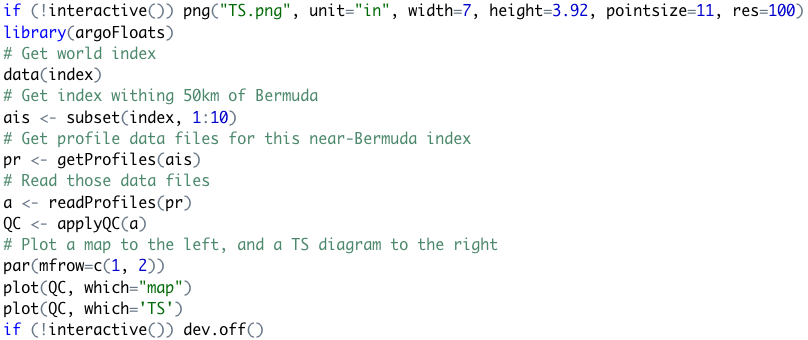
\includegraphics{../18_tweets/TScode.png}
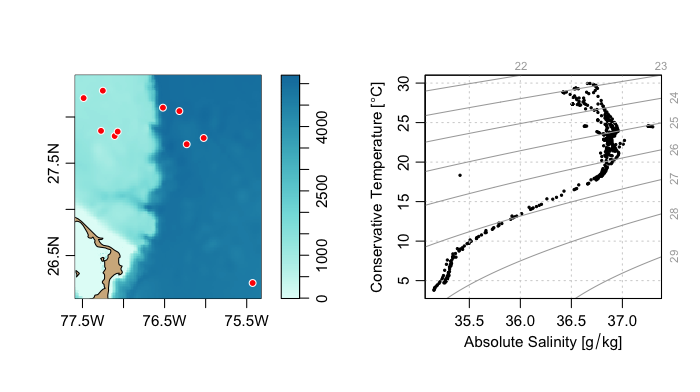
\includegraphics{../18_tweets/TS.png}

\hypertarget{tweet-6}{%
\section{Tweet 6}\label{tweet-6}}

To subset by ocean ``Area'', the following code is used. Note: we'e also
incorporated a subset by polygon to better improve this subset.

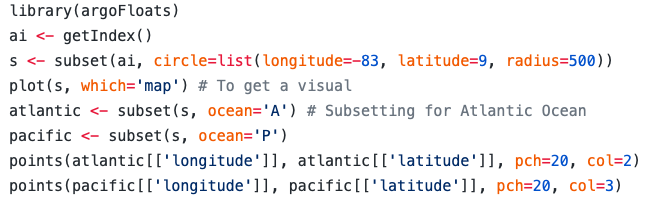
\includegraphics{../18_tweets/oceanAreaCode.png}
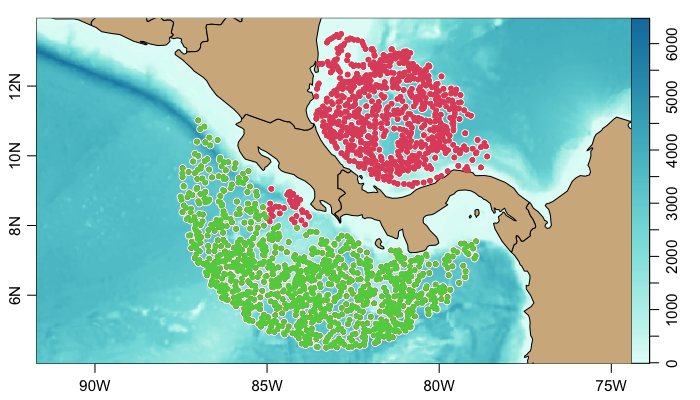
\includegraphics{../18_tweets/oceanArea.png}

\hypertarget{tweet-7}{%
\section{Tweet 7}\label{tweet-7}}

The code shown below demonstrates how to use our subset by polygon and
TS plot function to create a TS diagram comparing the Atlantic and
Pacific Ocean near the Isthmus of Panama.

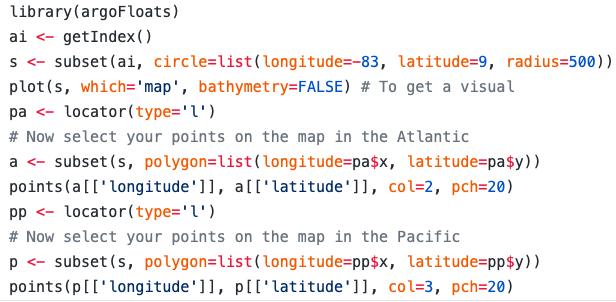
\includegraphics{../18_tweets/polygonCode.png}
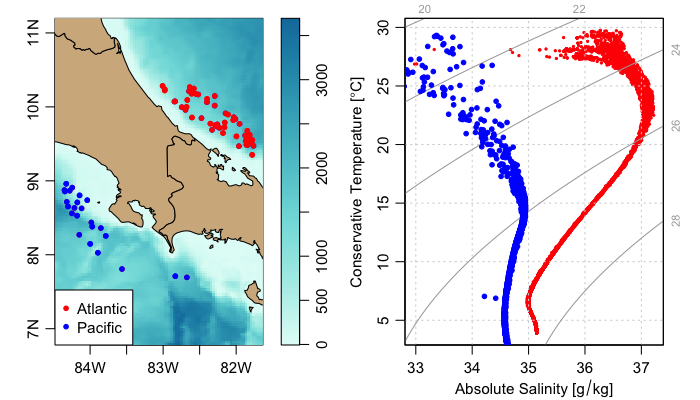
\includegraphics{../18_tweets/TSpanama.png}

\hypertarget{tweet-8}{%
\section{Tweet 8}\label{tweet-8}}

In addition, argoFloats users have the ability to create a TS diagram,
colour-coded by oxygen using the following code:

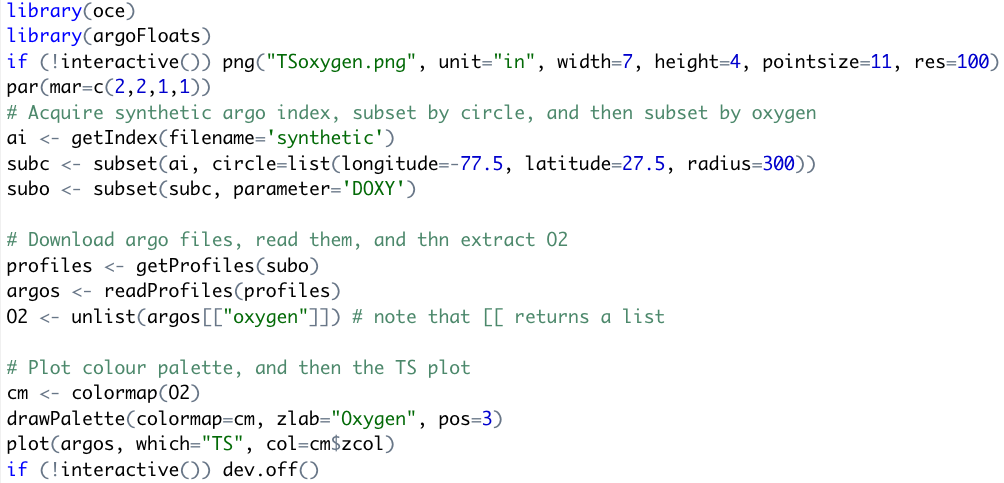
\includegraphics{../18_tweets/TSoxygenCode.png}

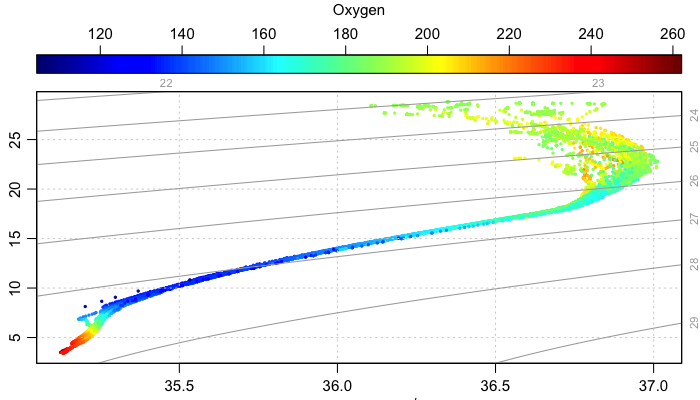
\includegraphics{../18_tweets/TSoxygen.png}

\hypertarget{tweet-9}{%
\section{Tweet 9}\label{tweet-9}}

Bathymetry has recently been added to the argoFloats package. A great
example of this is shown by this trajectory plot colour coded by time,
with bathymetry in the Labrador Sea.

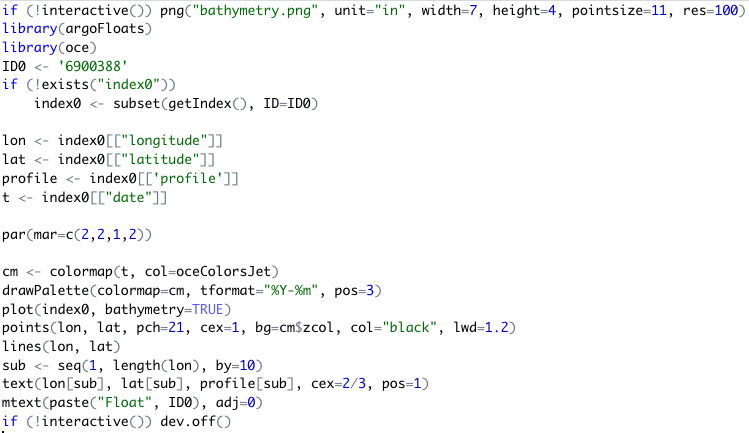
\includegraphics{../18_tweets/bathymetryCode.png}

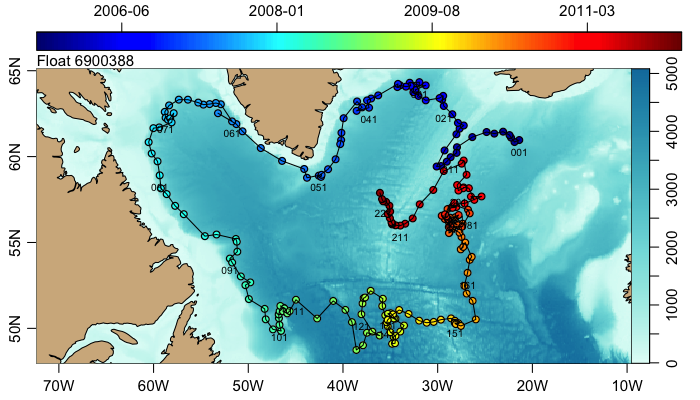
\includegraphics{../18_tweets/bathymetry.png}

\hypertarget{tweet-10}{%
\section{Tweet 10}\label{tweet-10}}

What about Quality Control (QC), you say? argoFloats has incorporated a
simple work flow to work with Argo float QC flags.

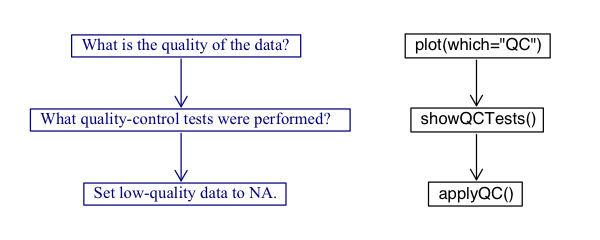
\includegraphics{../../../vignettes/qc_flowchart.png}

\hypertarget{tweet-11}{%
\section{Tweet 11}\label{tweet-11}}

The first phase when dealing with QC for Argo data is to plot the
quality of the data using the QC plot. This is shown in the code below
where each point is a cycle representing ``bad'' data in red, and
``good'' data in black.

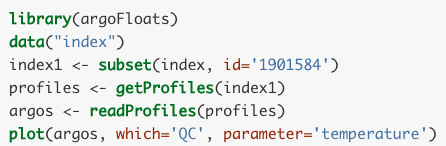
\includegraphics{../18_tweets/plotQCCode.png}
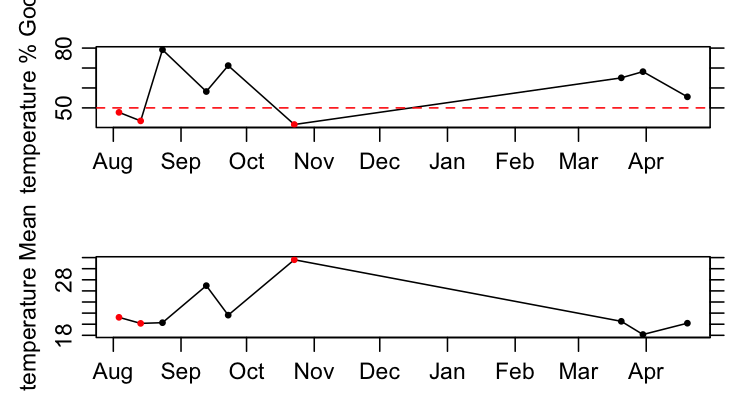
\includegraphics{../../../vignettes/plotqc.png}

\hypertarget{tweet-12}{%
\section{Tweet 12}\label{tweet-12}}

In the QC plot, the first cycle is considered ``bad''. To determine
which QC Tests were performed on that cycle the following code is used
to produce the following output:

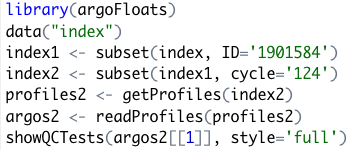
\includegraphics{../18_tweets/showQCTestsCode.png}
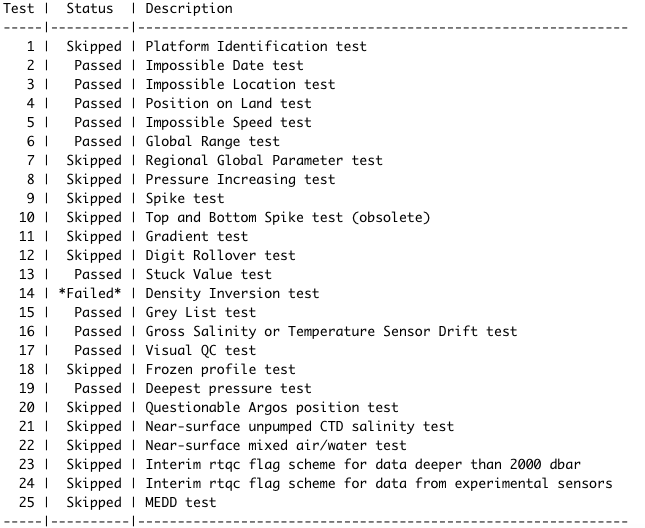
\includegraphics{../18_tweets/showQCTestOutput.png}

\#Tweet 13

If the user agrees with the test failed, they can replace all suspicious
data with NA. For example, the following code shows the need for QC
testing in our previous example.

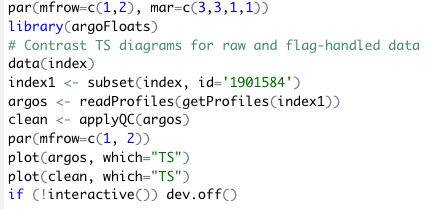
\includegraphics{../18_tweets/applyQCCode.png}
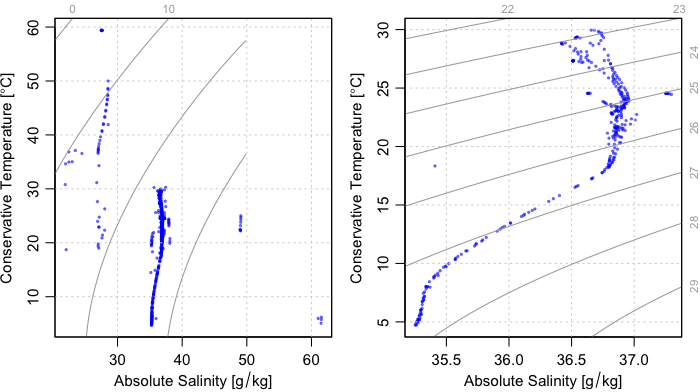
\includegraphics{../../../vignettes/applyQC.png}

\hypertarget{tweet-15}{%
\section{Tweet 15}\label{tweet-15}}

In addition to flags, some data sets undergo adjustments that are made
in recognition of the QC analysis or to employ information about
improved calibrations, etc. For this reason the useAdjusted function was
created.

\hypertarget{tweet-16}{%
\section{Tweet 16}\label{tweet-16}}

useAdjusted can be a fairly complicated process. However, the diagram
below demonstrates the actions taken when a user specifies
\texttt{which=ALL} or \texttt{which=\textless{}param\textgreater{}}.

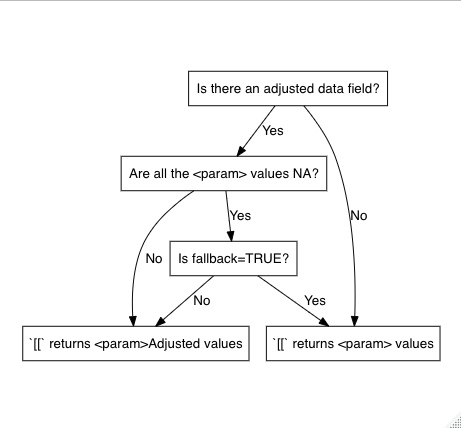
\includegraphics{../../../man/figures/useAdjustedDiagram.png}

\hypertarget{tweet-17}{%
\section{Tweet 17}\label{tweet-17}}

An example where useAdjusted is useful is when dealing with oxygen data.
Often times, BGC data need calibration due to sensors and that can be
represented in the data, as shown below.

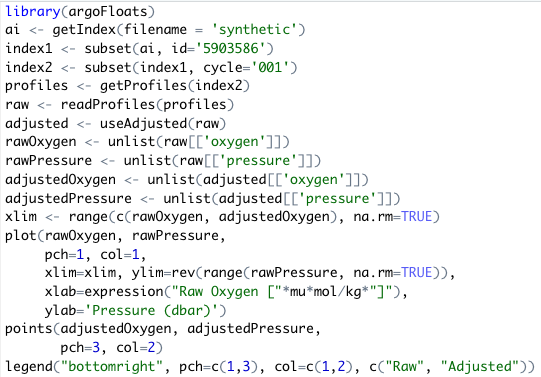
\includegraphics{../18_tweets/useAdjustedCode.png}
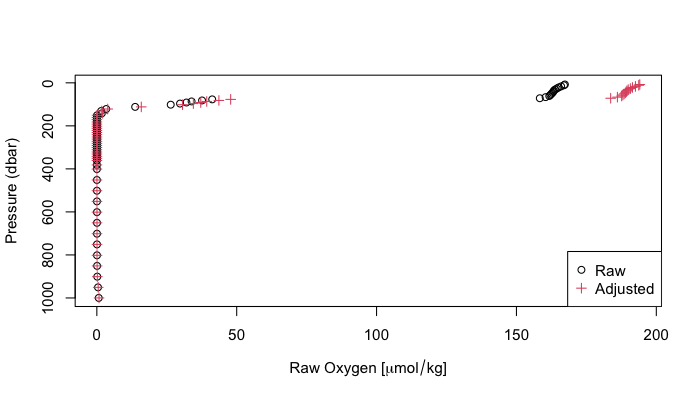
\includegraphics{../18_tweets/useAdjusted.png}

\end{document}
